% Created by tikzDevice version 0.12.3.1 on 2022-09-02 16:30:35
% !TEX encoding = UTF-8 Unicode
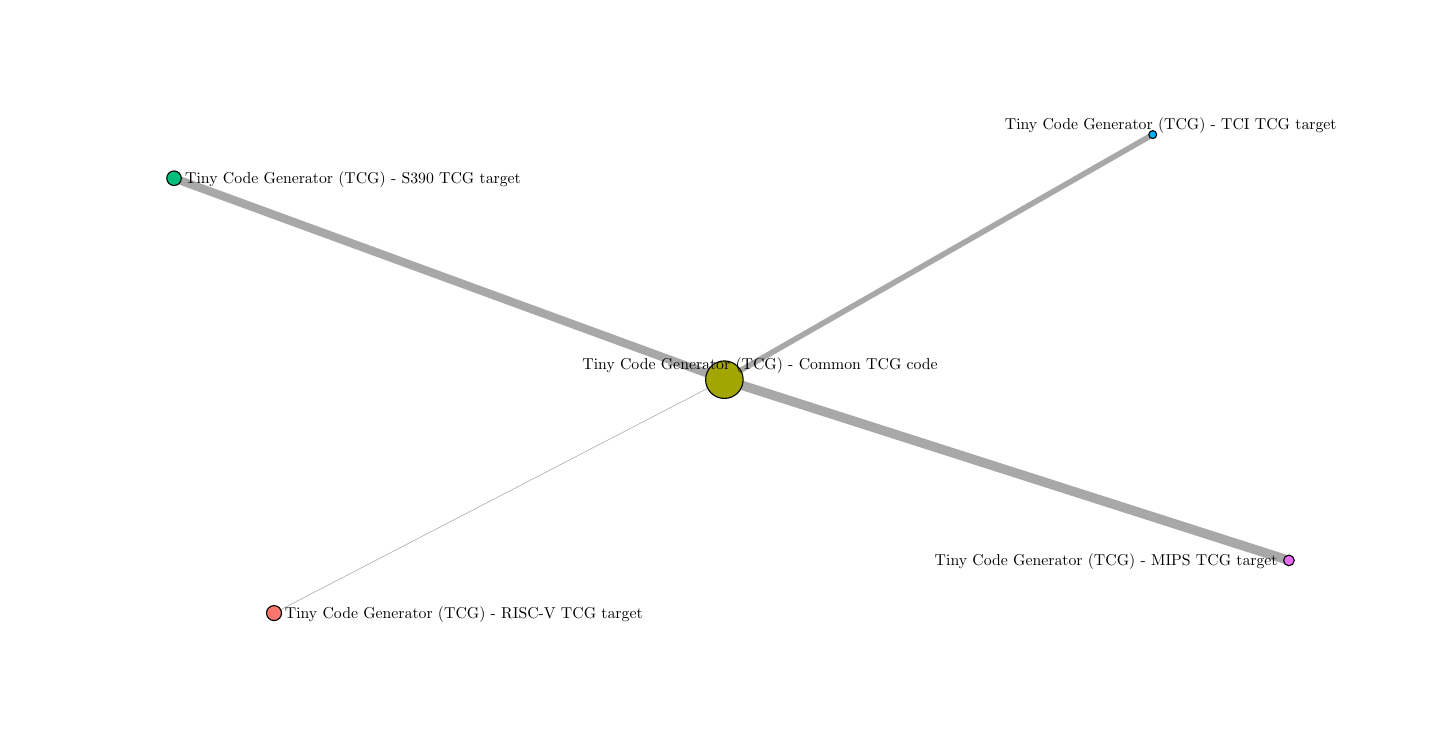
\begin{tikzpicture}[x=1pt,y=1pt]
\definecolor{fillColor}{RGB}{255,255,255}
\path[use as bounding box,fill=fillColor,fill opacity=0.00] (0,0) rectangle (505.89,252.94);
\begin{scope}
\path[clip] (  0.00,  0.00) rectangle (505.89,252.94);
\definecolor{fillColor}{RGB}{255,255,255}

\path[fill=fillColor] (  0.00,  0.00) rectangle (505.89,252.94);
\end{scope}
\begin{scope}
\path[clip] ( 32.75, 32.75) rectangle (475.89,222.94);
\definecolor{drawColor}{gray}{0.66}

\path[draw=drawColor,line width= 3.4pt,line join=round] (251.75,125.74) -- (455.75, 60.43);

\path[draw=drawColor,line width= 0.2pt,line join=round] (251.75,125.74) -- ( 89.02, 41.40);

\path[draw=drawColor,line width= 3.0pt,line join=round] (251.75,125.74) -- ( 52.89,198.53);

\path[draw=drawColor,line width= 2.0pt,line join=round] (251.75,125.74) -- (406.54,214.30);
\definecolor{drawColor}{RGB}{0,0,0}
\definecolor{fillColor}{RGB}{163,165,0}

\path[draw=drawColor,line width= 0.4pt,line join=round,line cap=round,fill=fillColor] (251.75,125.74) circle (  6.78);
\definecolor{fillColor}{RGB}{231,107,243}

\path[draw=drawColor,line width= 0.4pt,line join=round,line cap=round,fill=fillColor] (455.75, 60.43) circle (  1.93);
\definecolor{fillColor}{RGB}{248,118,109}

\path[draw=drawColor,line width= 0.4pt,line join=round,line cap=round,fill=fillColor] ( 89.02, 41.40) circle (  2.71);
\definecolor{fillColor}{RGB}{0,191,125}

\path[draw=drawColor,line width= 0.4pt,line join=round,line cap=round,fill=fillColor] ( 52.89,198.53) circle (  2.63);
\definecolor{fillColor}{RGB}{0,176,246}

\path[draw=drawColor,line width= 0.4pt,line join=round,line cap=round,fill=fillColor] (406.54,214.30) circle (  1.43);

\node[text=drawColor,anchor=base,inner sep=0pt, outer sep=0pt, scale=  0.57] at (264.66,129.33) {Tiny Code Generator (TCG) - Common TCG code};

\node[text=drawColor,anchor=base,inner sep=0pt, outer sep=0pt, scale=  0.57] at (389.72, 58.47) {Tiny Code Generator (TCG) - MIPS TCG target};

\node[text=drawColor,anchor=base,inner sep=0pt, outer sep=0pt, scale=  0.57] at (157.58, 39.43) {Tiny Code Generator (TCG) - RISC-V TCG target};

\node[text=drawColor,anchor=base,inner sep=0pt, outer sep=0pt, scale=  0.57] at (117.57,196.57) {Tiny Code Generator (TCG) - S390 TCG target};

\node[text=drawColor,anchor=base,inner sep=0pt, outer sep=0pt, scale=  0.57] at (413.05,216.01) {Tiny Code Generator (TCG) - TCI TCG target};
\end{scope}
\end{tikzpicture}
